%
% LaTeX report template 
%

% This is a comment: in LaTeX everything that in a line comes
% after a "%" symbol is treated as comment

\documentclass[11pt, a4paper]{article}
\usepackage{graphicx}
\usepackage{amsmath}
\usepackage{listings}


\title{Assignment 3} % Title

\author{Om Shri Prasath (EE17B113)} % Author name

\date{\today} % Date for the report
\begin{document}		
		
\maketitle % Insert the title, author and date
\section{Aim of Assignment}
%Create new section;it is autonumbered

 In this assignment we aim to :
 \begin{itemize}
     \item Observe the error of trying to find the least error fit function for a data due to noise.
     \item Find the relation between the error and the noise.
 \end{itemize}

\section{Procedure}
The function to be fitted is :
\begin{equation*}
    f(t) = 1.05J_2(t)-0.105t
\end{equation*}
The true data is collected from the above function.
\subsection{Creating noisy data}
    To create the noisy data, we add random noise to the function. This random noise (denoted by \textit{n}(\textit{t})))
    is given by the normally distributed probability function :
    \begin{equation*}
        Pr(n(t)|\sigma)=\frac{1}{\sigma\sqrt{2\pi}}exp\left(-\frac{n(t)^2}{2\sigma^2}\right)
    \end{equation*}
    Where $\sigma$ is generated in code implementation as :
    \begin{lstlisting}
        sigma = logspace(-1,-3,9)
    \end{lstlisting}
Thus the resulting noisy data will be of the form :
\begin{equation*}
    f(t) = 1.05J_2(t)-0.105t+n(t)
\end{equation*}
Thus for 9 different values of sigma, the noisy data is created and stored in the \textit{\textbf{fitting.dat}} file
\subsection{Analyzing the noisy data}
The data is read into a Python code and is plotted using PyPlot. The output result looks as follows:
   \begin{figure}[!tbh]
   	\centering
   	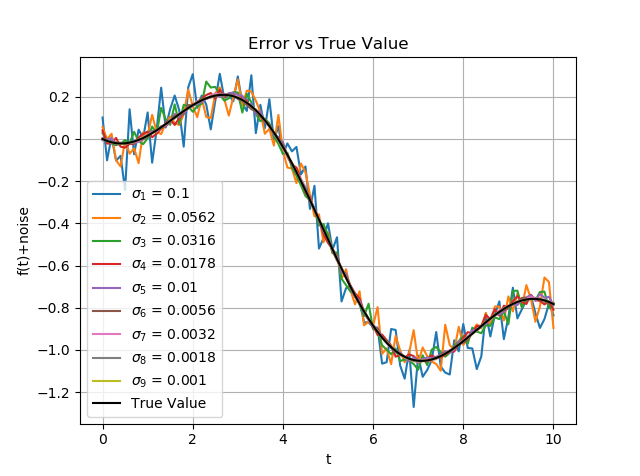
\includegraphics[scale=0.5]{./../Extras/NoisewithTrue.png}  % Mention the image name within the curly braces. Image should be in the same folder as the tex file. 
       \caption{Noisy Data With the True Data}
   	\label{fig:noisytrue}
   \end{figure}
\\As we can see, the noisiness in the data increases with increasing value of $\sigma$. Another view of how the noise affects the data can be seen below :
   \begin{figure}[!tbh]
    \centering
    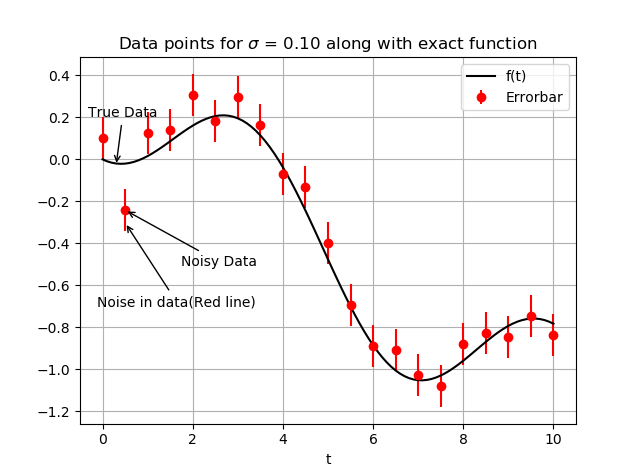
\includegraphics[scale=0.5]{./../Extras/NoiseErrorbar.png}  % Mention the image name within the curly braces. Image should be in the same folder as the tex file. 
    \caption{Noisy Data with Errorbar}
    \label{fig:noiseerr}
\end{figure}
\\The red lines indicate the standard deviation of the noisy data from the original data.
\subsection{Finding the best approximation for the noisy data}
From the data, we can conclude that the data can be fitted into a function of the form :
\begin{equation*}
    f(t) = AJ_2(t)+Bt
\end{equation*}
To find the coefficients \textit{A} and \textit{B}, we first try to find the mean square error between the function and the data for a range of values of \textit{A} and \textit{B}
, which is given by :
\begin{equation*}
\epsilon_{ij} = \frac{1}{101}\sum_{k=0}^{101}(f_k - g(t_k,A_i,B_j))^2
\end{equation*}
where $\epsilon_{ij}$ is the error for $(A_i,B_j)$ set. The contour plot of the error is shown below :
\begin{figure}[!tbh]
    \centering
    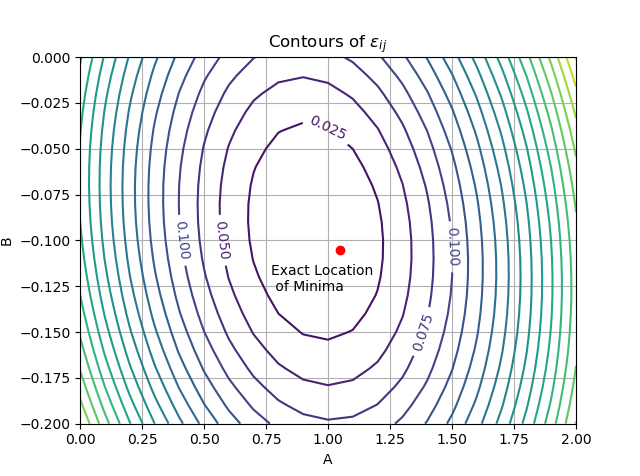
\includegraphics[scale=0.5]{./../Extras/Contour.png}  % Mention the image name within the curly braces. Image should be in the same folder as the tex file. 
    \caption{Contour Plot of $\epsilon_{ij}$}
    \label{fig:contour}
\end{figure}
\\We can see the location of the minima to be approximately near the orignal function coefficients
Now we solve for the function using the \texttt{lstsq} function in Python for the equation 
$M.p = D$ for $p$ where $M=\left[\begin{matrix}
    J_2(t_1)&t_1\\
    ...&...\\
    J_2(t_m)&t_m
\end{matrix}\right]$
, $p=\left[\begin{matrix}
    A_o\\B_o
\end{matrix}\right]$
and $D$ is the column matrix of the noisy data.
\\\\\\\\\\\\\\\\\\Thus, we solve for $p$ and then find the mean square error of the values of $A$ and $B$ found using \texttt{lstsq} and the original values (1.05,-0.105). \\The plot for the different noisy data is as follows :
\begin{figure}[!tbh]
    \centering
    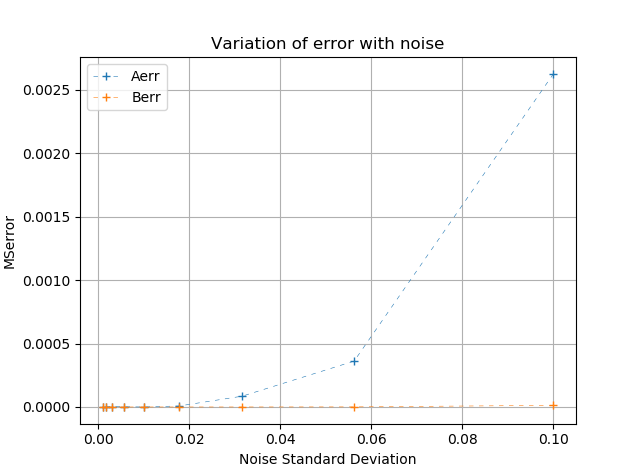
\includegraphics[scale=0.5]{./../Extras/ErrorwithStd.png}  % Mention the image name within the curly braces. Image should be in the same folder as the tex file. 
    \caption{Error vs Standard Deviation}
    \label{fig:errorstd}
\end{figure}
\\This plot does not give that much useful information between $\sigma$ and $\epsilon$, but when we do the \texttt{loglog} plot as below :
\begin{figure}[!tbh]
    \centering
    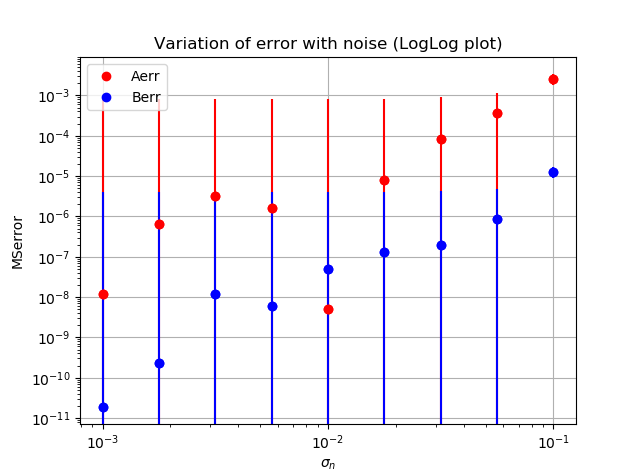
\includegraphics[scale=0.5]{./../Extras/ErrorWithStdLogLog.png}  % Mention the image name within the curly braces. Image should be in the same folder as the tex file. 
    \caption{Error vs Standard Deviation loglog Plot}
    \label{fig:errorstdlog}
\end{figure}
\\We can see an approximate linear relation between $\sigma$ and $\epsilon$. This is the required result.
\section{Conclusion}
From the above procedure, we were able to determine that the \textbf{logarithm of the noise} \textit{\textbf{linearly affects}}  the \textbf{logarithm of the error} in the calcuation of the \textbf{least error fit} for a given data
\end{document}